% Hlavicka pro protokoly z fyzikalniho praktika.
% Verze pro: LaTeX
% Verze hlavicky: 22. 2. 2007
% Autor: Ustav fyziky kondenzovanych latek
% Ke stazeni: www.physics.muni.cz/ufkl/Vyuka/
% Licence: volne k pouziti, nejlepe k vcasnemu odevzdani protokolu z Vaseho mereni.

\documentclass[a4paper,11pt]{article}

% Kodovani (cestiny) v dokumentu: cp1250
% \usepackage[cp1250]{inputenc}	% Omezena stredoevropska kodova stranka, pouze MSW.
\usepackage[utf8]{inputenc}	% Doporucujeme pouzivat UTF-8 (unicode).

%%% Nemente:
\usepackage[margin=2cm]{geometry}
\newtoks\jmenopraktika \newtoks\jmeno \newtoks\datum
\newtoks\obor \newtoks\skupina \newtoks\rocnik \newtoks\semestr
\newtoks\cisloulohy \newtoks\jmenoulohy
\newtoks\tlak \newtoks\teplota \newtoks\vlhkost
%%% Nemente - konec.


%%%%%%%%%%% Doplnte pozadovane polozky:

\jmenopraktika={Fyzikální praktikum 1}  % nahradte jmenem vaseho predmetu
\jmeno={Milan Suk}            % nahradte jmenem mericiho
\datum={12. března 2018}        % nahradte datem mereni ulohy
\obor={F}                     % nahradte zkratkou vami studovaneho oboru
\skupina={PO 8:00}            % nahradte dobou vyuky vasi seminarni skupiny
\rocnik={I}                  % nahradte rocnikem, ve kterem studujete
\semestr={II}                 % nahradte semestrem, ve kterem studujete

\cisloulohy={6}               % nahradte cislem merene ulohy
\jmenoulohy={Tepelné vlastnosti kapalin - elektrický kalorimetr} % nahradte jmenem merene ulohy

\tlak={97,9}                   % nahradte tlakem pri mereni (v hPa)
\teplota={21,4}               % nahradte teplotou pri mereni (ve stupnich Celsia)
\vlhkost={40}               % nahradte vlhkosti vzduchu pri mereni (v %)

%%%%%%%%%%% Konec pozadovanych polozek.


%%%%%%%%%%% Uzitecne balicky:
\usepackage[czech]{babel}
\usepackage{graphicx}
\usepackage{amsmath}
\usepackage{xspace}
\usepackage{url}
\usepackage{indentfirst}
\usepackage{listings}
\usepackage{color}


\definecolor{codegreen}{rgb}{0,0.6,0}
\definecolor{codegray}{rgb}{0.5,0.5,0.5}
\definecolor{codepurple}{rgb}{0.58,0,0.82}
\definecolor{backcolour}{rgb}{0.95,0.95,0.92}
 
\lstdefinestyle{mystyle}{
    backgroundcolor=\color{backcolour},   
    commentstyle=\color{codegreen},
    keywordstyle=\color{magenta},
    numberstyle=\tiny\color{codegray},
    stringstyle=\color{codepurple},
    basicstyle=\footnotesize,
    breakatwhitespace=false,         
    breaklines=true,                 
    captionpos=b,                    
    keepspaces=true,                 
    numbers=left,                    
    numbersep=5pt,                  
    showspaces=false,                
    showstringspaces=false,
    showtabs=false,                  
    tabsize=2
}
 
\lstset{style=mystyle}

%%%%%% Zamezeni parchantu:
\widowpenalty 10000 \clubpenalty 10000 \displaywidowpenalty 10000
%%%%%% Parametry pro moznost vsazeni vetsiho poctu obrazku na stranku
\setcounter{topnumber}{3}	  % max. pocet floatu nahore (specifikace t)
\setcounter{bottomnumber}{3}	  % max. pocet floatu dole (specifikace b)
\setcounter{totalnumber}{6}	  % max. pocet floatu na strance celkem
\renewcommand\topfraction{0.9}	  % max podil stranky pro floaty nahore
\renewcommand\bottomfraction{0.9} % max podil stranky pro floaty dole
\renewcommand\textfraction{0.1}	  % min podil stranky, ktery musi obsahovat text
\intextsep=8mm \textfloatsep=8mm  %\intextsep pro ulozeni [h] floatu a \textfloatsep pro [b] or [t]

% Tecky za cisly sekci:
\renewcommand{\thesection}{\arabic{section}.}
\renewcommand{\thesubsection}{\thesection\arabic{subsection}.}
% Jednopismenna mezera mezi cislem a nazvem kapitoly:
\makeatletter \def\@seccntformat#1{\csname the#1\endcsname\hspace{1ex}} \makeatother


%%%%%%%%%%%%%%%%%%%%%%%%%%%%%%%%%%%%%%%%%%%%%%%%%%%%%%%%%%%%%%%%%%%%%%%%%%%%%%%
%%%%%%%%%%%%%%%%%%%%%%%%%%%%%%%%%%%%%%%%%%%%%%%%%%%%%%%%%%%%%%%%%%%%%%%%%%%%%%%
% Zacatek dokumentu
%%%%%%%%%%%%%%%%%%%%%%%%%%%%%%%%%%%%%%%%%%%%%%%%%%%%%%%%%%%%%%%%%%%%%%%%%%%%%%%
%%%%%%%%%%%%%%%%%%%%%%%%%%%%%%%%%%%%%%%%%%%%%%%%%%%%%%%%%%%%%%%%%%%%%%%%%%%%%%%

\begin{document}

%%%%%%%%%%%%%%%%%%%%%%%%%%%%%%%%%%%%%%%%%%%%%%%%%%%%%%%%%%%%%%%%%%%%%%%%%%%%%%%
% Nemente:
%%%%%%%%%%%%%%%%%%%%%%%%%%%%%%%%%%%%%%%%%%%%%%%%%%%%%%%%%%%%%%%%%%%%%%%%%%%%%%%
\thispagestyle{empty}

{
\begin{center}
\sf 
{\Large Ústav fyzikální elektroniky Přírodovědecké fakulty Masarykovy univerzity} \\
\bigskip
{\huge \bfseries FYZIKÁLNÍ PRAKTIKUM} \\
\bigskip
{\Large \the\jmenopraktika}
\end{center}

\bigskip

\sf
\noindent
\setlength{\arrayrulewidth}{1pt}
\begin{tabular*}{\textwidth}{@{\extracolsep{\fill}} l l}
\large {\bfseries Zpracoval:}  \the\jmeno & \large  {\bfseries Naměřeno:} \the\datum\\[2mm]
\large  {\bfseries Obor:} \the\obor  \hspace{40mm}  {\bfseries Skupina:} \the\skupina %
&\large {\bfseries Testováno:}\\
\\
\hline
\end{tabular*}
}

\bigskip

{
\sf
\noindent \begin{tabular}{p{3cm} p{0.6\textwidth}}
\Large  Úloha č. {\bfseries \the\cisloulohy:} \par
&\Large \bfseries \the\jmenoulohy  \\[2mm]
\end{tabular}
}

%%%%%%%%%%%%%%%%%%%%%%%%%%%%%%%%%%%%%%%%%%%%%%%%%%%%%%%%%%%%%%%%%%%%%%%%%%%%%%%
% konec Nemente.
%%%%%%%%%%%%%%%%%%%%%%%%%%%%%%%%%%%%%%%%%%%%%%%%%%%%%%%%%%%%%%%%%%%%%%%%%%%%%%%

%%%%%%%%%%%%%%%%%%%%%%%%%%%%%%%%%%%%%%%%%%%%%%%%%%%%%%%%%%%%%%%%%%%%%%%%%%%%%%%
%%%%%%%%%%%%%%%%%%%%%%%%%%%%%%%%%%%%%%%%%%%%%%%%%%%%%%%%%%%%%%%%%%%%%%%%%%%%%%%
% Zacatek textu vlastniho protokolu
%%%%%%%%%%%%%%%%%%%%%%%%%%%%%%%%%%%%%%%%%%%%%%%%%%%%%%%%%%%%%%%%%%%%%%%%%%%%%%%
%%%%%%%%%%%%%%%%%%%%%%%%%%%%%%%%%%%%%%%%%%%%%%%%%%%%%%%%%%%%%%%%%%%%%%%%%%%%%%%


\section{Úvod, postup měření}

    \paragraph{} Cílem tohoto měření bylo měřit tepelné vlastnosti kapalin.
    Konkrétně jsem měřil kapacitu kalorimetru, ve kterém jsem posléze
    \textit{mtodou 1} měřil keofecient chladnutí $\beta$.

    \subsection{Kalorimetr}

        \paragraph{} Kapacitu kalorimetru jsem určil pomocí dvou stejných kapalin
        o různých počítačních teplotách a hmotnostech. Ty se smísili v kalorimetru
        a vyrovnali celkovou teplotu na $t$. Ze známých počátečních teplot $t_1$ a
        $t_2$, hmotnost9 $m_1$ a $m_2$ měrné tepelné kapacity vody $c$ lze 
        kapacitu kalorimetru vypočíst pomocí rovnice (1).

        \begin{equation}
            K = c \left[ m_2 \frac{t_2 - t}{t - t_1} - m_1 \right]
        \end{equation}


        \paragraph{} Nejistotu měření určím ze \textit{Zákona šíření nejistoty} jako

        $$
        u(K) = \sqrt{
          \left(\frac{\partial K}{\partial m_1}\right)^{2} \cdot u(m)^{2}
        + \left(\frac{\partial K}{\partial m_2}\right)^{2} \cdot u(m)^{2} 
        + \left(\frac{\partial K}{\partial t}\right)^{2} \cdot u(t)^{2}
        + \left(\frac{\partial K}{\partial t_1}\right)^{2} \cdot u(t)^{2}
        + \left(\frac{\partial K}{\partial t_2}\right)^{2} \cdot u(t)^{2}
        }
        $$

        \begin{equation}
        = \sqrt{
              \left(u(m) \cdot c\right)^{2}
            + \left(\frac{c \cdot u(m) \cdot (t_2 - t)}{(t - t_1)^{2}}\right)^{2}
            + \left(\frac{c \cdot m_2 \cdot u(t) \cdot (t_2 - t)}{\left(t - t_1\right)^{2}}\right)^{2}
            + ...
        }
        \end{equation}

    \subsection{Koeficient chladnutí $\beta$}

        \paragraph{} Metoda 1 je založená na exponenciální závislosti 
        teploty na čas podle rovnice (3).

        \begin{equation}
            t(\tau) = t_{o} + (t_{p} - t_{o}) e^{-\frac{\beta}{mc + K} \tau}
        \end{equation}

        \paragraph{} Naměřená data bude potřeba fitovat na o konstantu
        posunutou exponencielu. Logaritmováním rovnice (3) získám následující
        tvar, který je již vhodný pro fitování na lineární funkci.
        
        $$
            ln(t - t_0) = ln(t_p - t_o) - \frac{\beta}{mc + K} \tau
        $$

        \paragraph{} Keoficient B získaný při fitování bude odpovídat
        členu $\frac{\beta}{mc + K}$. Konečný výsledek získám jako

        $$
            \beta = - B \cdot (mc + K)
        $$

\section{Zpracování měření}

    \paragraph{} Kapacitu kalorimetru určím pomocí následujícího python
    skriptu.

    \begin{lstlisting}[language=Python]
import math

m1 = 0.174631
t1 = 21.2
m2 = 0.178321
t2 = 72.6
t = 42.8
c = 4180

K = m2 * c * (t2 - t) * 1 / (t - t1) - m1 * c

ut = 0.1
um = 0.0000005

uK = math.sqrt(
    math.pow(c, 2) * math.pow(um, 2) +
    math.pow(c * (t2 - t) / (t - t1), 2) * math.pow(um, 2) +
    math.pow(c * m2 / (t - t1), 2) * math.pow(ut, 2) +
    math.pow(c * m2 * (t2 - t) / math.pow((t - t1), 2), 2) * math.pow(ut, 2) +
    math.pow(c * m2 * (t1 - t2) / math.pow((t - t1), 2), 2) * math.pow(ut, 2)
)

print("K = {} +- {}".format(K, uK))\end{lstlisting}

    \begin{lstlisting}[language=Bash]
> python3 regrese.py 
K = 298.3932090740741 +- 10.099839355542386 \end{lstlisting}


    \paragraph{} Fitování za mě udělá balíček \textit{numpy}. V rámci
    pythnovského skriptu také generuji modelové řešení pro porovnání
    s naměřenými daty.

    \begin{lstlisting}[language=Python]
import numpy as np
import sys

file_data = np.loadtxt(sys.argv[1])

m = 0.174631
c = 4180
K = 290

t_0 = 21
t_p = file_data[0][1]

y = [x[1] for x in file_data]
y_log = [np.log(x[1] - t_0) for x in file_data]
x = [x[0] * 60 for x in file_data]

fit = np.polyfit(x, y_log, 1)
beta = - fit[0] * (m * c + K)

print("beta = ", beta)

import matplotlib.pyplot as plot

prediction_x = x
prediction_y = [np.exp(fit[0] * t) * np.exp(fit[1]) + t_0 for t in x]

fig, plots = plot.subplots()

plots.plot(x, y, 'r--', label="namereno")
plots.plot(prediction_x, prediction_y, 'b--', label="model")

plot.legend()
plot.ylabel("cas [s]")
plot.xlabel("templota [C]")
plot.show()\end{lstlisting} 

    \begin{lstlisting}[language=Bash]
> python3 regrese.py data1.txt
beta = 0.3614100256292938
> python3 regrese.py data2.txt
beta = 0.26066540522960097
\end{lstlisting}

    \paragraph{} Vygenerované grafy jsou přiloženy níže.

    \begin{figure}[h!]
        \centering
        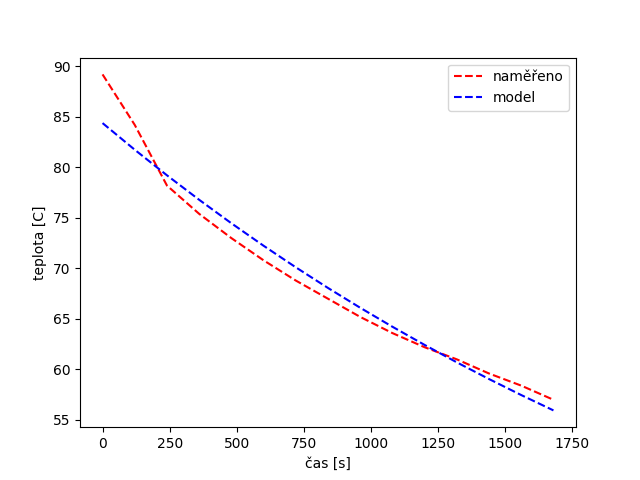
\includegraphics[width=0.7\linewidth]{data1.png}
        \caption{data1.txt}
        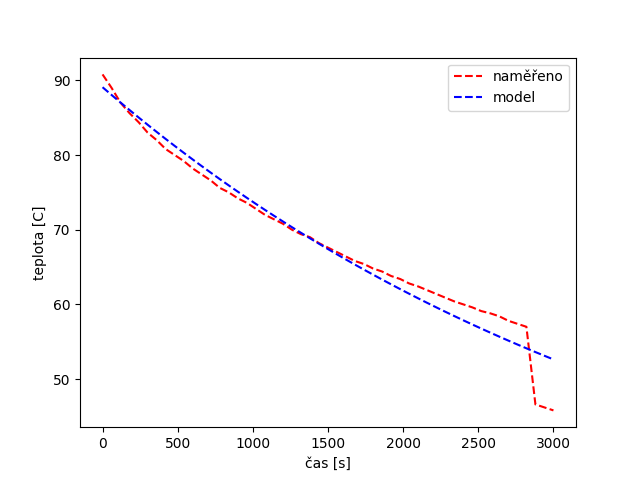
\includegraphics[width=0.7\linewidth]{data2.png}
        \caption{data2.txt}
    \end{figure}

\section{Zhodnocení měření, závěr}

    \paragraph{} Kapacita kalorimetru vyšla docela rozumně $K = 300 \pm 10 J \cdot kg^{-1}$.
    Zajímavé josu číselné hodnoty $\beta$. V prvním případě, kdy bylo měření prováděno
    v samotném kalorimetru, vyšla hodnota o desetinu méně, než při druhém měření,
    kdy byl kalorimetr ještě obalem ve válci, který mu dodával na izolaci. Rozdíl
    je asi ne místě, protože je izolujícím válcem omezen kontakt s okolím a 
    tepelná výměna probíha pomaleji.

\end{document}
